\documentclass{ctexart}
\usepackage{indentfirst}
\usepackage{array}
\usepackage{graphicx}
\usepackage{url}
\graphicspath{ {images/} }
\begin{document}

\title{基于ARM架构的超低功耗OS可行性报告}
\author{崔天一\ 曹焕琦\ 邓翔\ 李泽昌}
\date{\today}
\begin{abstract}
 本文简要论证了将uC/OS移植到蓝牙DA14580并实现低功耗且正常使用DA14580蓝牙协议栈的可行性,并描述了该种做法的创新点。本文依次介绍了uC/OS移植的一般步骤,外部中断的处理方法,休眠的实现方法。
\end{abstract}

\maketitle

\tableofcontents
\newpage
\section{uC/OS II的移植\cite{001}}
\subsection{移植条件}
要移植uC/OS,处理器需满足以下条件。
\begin{enumerate}
\item 处理器的C编译器能够产生可重入型的代码
\item 处理器支持定时中断
\item 可以使用C语言开关中断
\item 处理器支持一定数量的数据存储硬件堆栈,可能需要几KB
\item 处理器上的指令支持将堆栈指针以及其他CPU寄存器中的内容读出,并存储到相应的内存或堆栈中
\end{enumerate}

开发过程中将使用Keil作为开发工具,编译器为ARMCC,满足以上编译器的需求。开发版支持32KHZ的实时钟,且拥有42KB的System SRAM,也有相应的存取指令,满足要求。
\subsection{移植细节}

\centerline{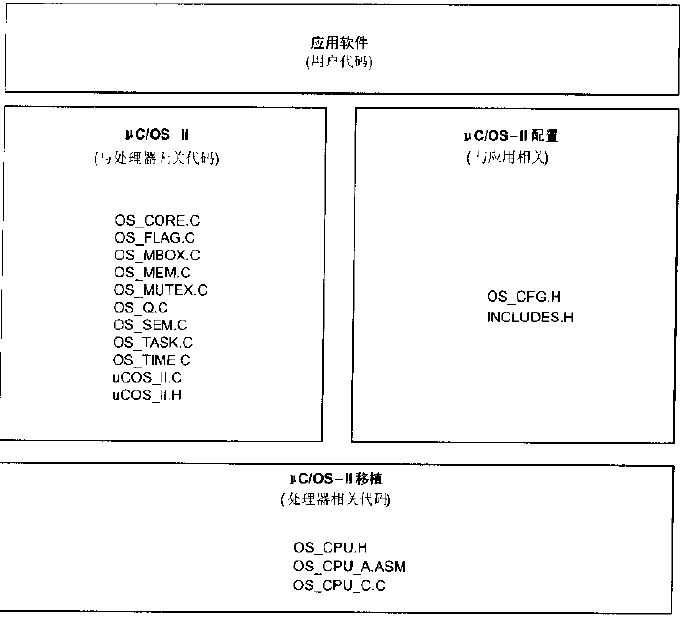
\includegraphics[scale=0.65]{001}}\par

在uC/OS的移植中,图中所示的与处理器无关的代码可以不用修改,移植到开发板上之后就可以利用里面支持的一些uC/OS的特性。可以看到,有三个文件OS\_CPU.H、OS\_CPU\_A.ASM和OS\_CPU\_C.C是需要我们根据处理器修改的。
\subsubsection{OS\_CPU.H}
不同的处理器支持的字长不同,所以需要定义不同的数据类型。

\centerline{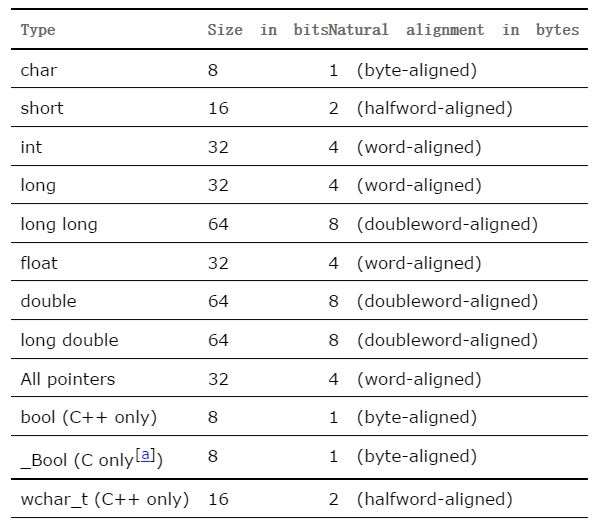
\includegraphics[scale=0.65]{002}}\par

根据编译器支持的数据类型,定义相应的uC/OS数据类型,如整形,浮点型及任务堆栈的数据类型,如果使用了一种特定的开关中断的方式,还需要声明CPU的状态寄存器的数据类型。

        除此之外,还需要定义OS\_ENTER\_CRITICAL()和OS\_EXIT\_CRITICAL()这两个宏,uC/OS使用这两个宏来开关中断。具体实现有三种。
        
        第一种方法是通过调用处理器的指令来开关中断。但在这种情况下,关闭中断后调用功能函数,返回时中断可能已被开启。比如,在一个中断子程序中,先关闭了中断,在退出时再开启中断。但是在中间的用户代码里调用了一个功能函数,该功能函数在进入时关闭中断,退出时开启中断,这样在退出中断子程序前中断就被开启了。
        
        第二种方法与第一种的区别是,在功能函数关中断前先将中断状态保存到堆栈,最后功能函数退出时不是开启中断,而是恢复原来的保存到堆栈中的中断状态,这样调用功能函数后就不会改变中断状态了。但如果编译器对插入汇编优化的得不够好的话,编译器可能不会知道堆栈指针已经因为保存了中断状态而改变,这样的话,所有变量的栈偏移量可能会偏差。
        
        第三种方法是利用编译器的扩展功能,将当前处理器状态字的值保存在局部变量里,最后用这个局部变量来恢复。
        
\centerline{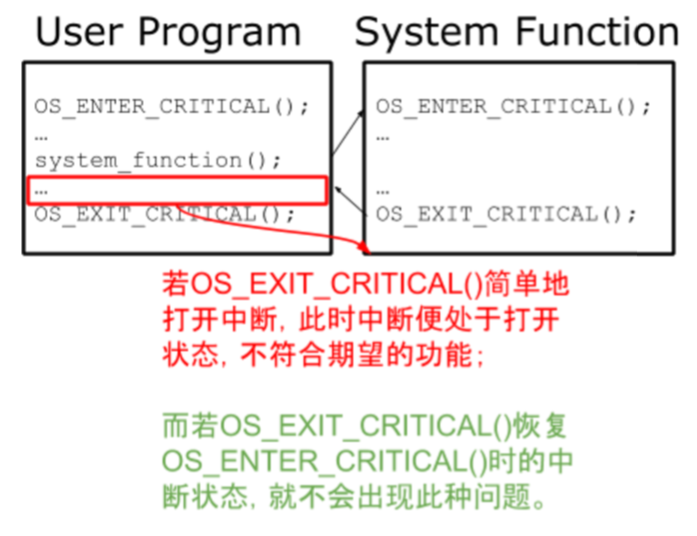
\includegraphics[scale=0.65]{interrupt}}\par
         
        变量OS\_STK\_GROWTH表示堆栈使用方向,设置为1表示高地址往低地址递减,0则相反。
               
        从低优先级任务切换到高优先级任务时需要调用OS\_TASK\_SW()宏。处于就绪态的任务的寄存器被保存在堆栈中,就像刚发生了中断一样。执行就绪态的任务,也就意味着恢复一系列的寄存器,并执行中断返回指令。这个宏就是用来模拟中断的产生。一般的处理器支持软中断或TRAP来完成这项操作,做法是让中断向量指向一个在OS\_CPU\_A.ASM中定义的任务级切换函数OSCtxSW(),或者调用它。
\subsubsection{OS\_CPU\_C.C}
这个文件中需要编写10个c语言函数。

\centerline{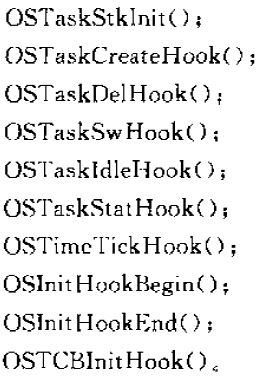
\includegraphics[scale=0.65]{003}}\par

但必须编写的只有OSTaskStkInit()函数,其余只要声明,不必包含内容。

该函数初始化堆栈结构,完成如下工作。

\centerline{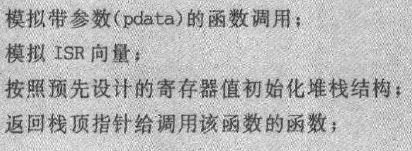
\includegraphics[scale=0.65]{004}}\par

以下是一个具体例子\cite{blog}

\centerline{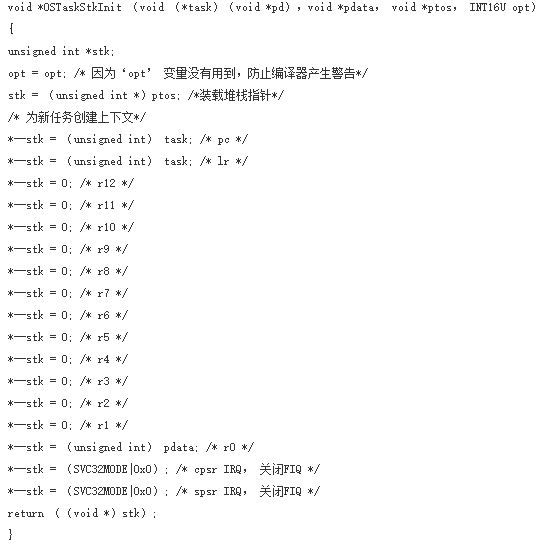
\includegraphics[scale=0.75]{example}}\par

\subsubsection{OS\_CPU\_A.ASM}
 这里需要编写4个汇编函数。
 
 OSStartHighRdy()用于使任务优先级最高的任务运行。该函数首先调用OSTaskSwHook(),这由用户在OS\_CPU\_C.c中自己定义。然后设置OSRunning为TRUE。接着获取优先级最高的任务的堆栈指针,恢复其所有的寄存器。
        
         OSCtxSw()是一个任务级的任务切换函数。首先保存寄存器到堆栈,再把堆栈指针存到当前任务的TCB里,然后调用OS\_CPU\_C.c中自己定义的OSTaskSwHook()函数。接着指向当前任务的指针的值改变,指向要恢复的任务,获取优先级,堆栈指针,按与保存时相反的方向恢复寄存器。
        
        OSTickISR()函数里由用户提供周期性地时钟源。可以在OSStart()运行后的第一个任务中初始化节拍中断。这个函数需要同其他中断服务子程序一样,设置OSIntNesting等等,它的用户代码就是调用OSTimeTick()。
        
         最后一个是OSIntCtxSw()。该函数在ISR中被OSIntExit()调用,因此假定所有寄存器都已保存,比起OSCtxSw()只是少了保存处理器的代码。
\section{中断处理程序(ISR)的编写}
\subsection{中断服务程序简介}
在移植过程中,我们不可避免的需要完成一些中断服务程序的编写(Interrupt Service Routine)。中断服务程序是一系列中断发生时CPU会跳转到的函数。如下为一个时钟中断处理函数:

\centerline{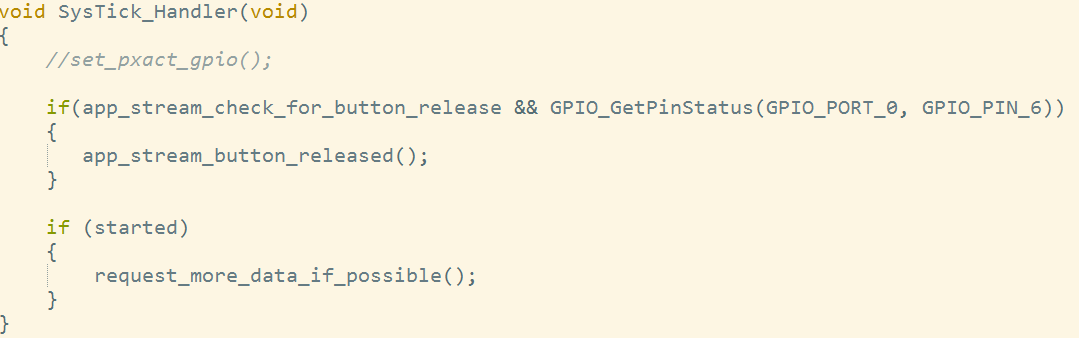
\includegraphics[scale=0.45]{005}}\par
事实上,开发板上所有具有的中断都在其官方提供的SDK包中的启动初始化代码boot\_vector.s中有所体现,如下图所示:

\centerline{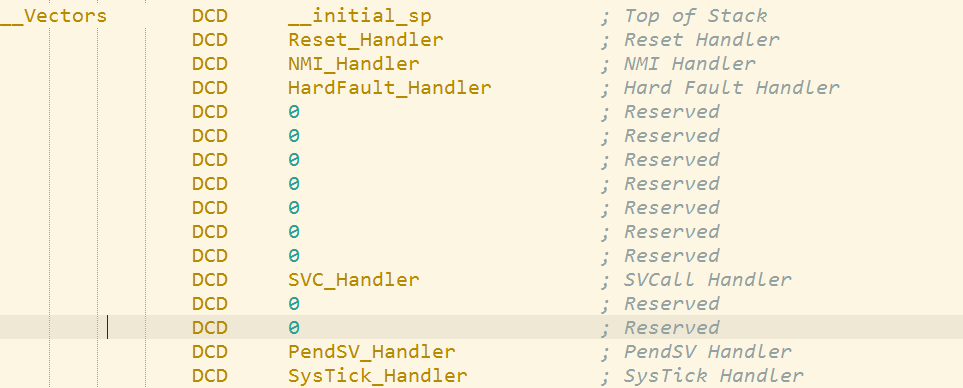
\includegraphics[scale=0.5]{006}}\par

所需的中断处理程序也可分为两部分:由ARM Cortex-M0定义的handler和由开发厂商定义的handler,上图所示的就是由Cortex-M0所定义的handler。

通过观察boot\_vector.s我们发现,它本身为全部的handler定义了符号位置,但导出到全局时仅是WEAK导出,因此当有C语言程序中包含了初始化汇编程序所定义的Handler的同名函数时,链接时对应的符号就会被填充上对应的函数的地址,否则会指向boot\_vector.s中的符号位置,此处仅有一条B .指令和一条ENDP指令,不响应中断直接跳回原位。

\centerline{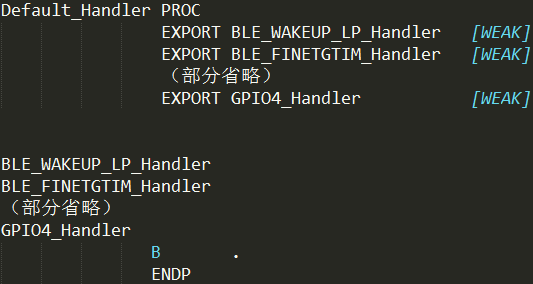
\includegraphics[scale=0.75]{007}}\par

因此,我们在移植完uC/OS II操作系统之后,只需定义对应名称的中断函数即可实现对应的中断功能。
\subsection{uC/OS II中应用程序使用中断的方式}
通常在嵌入式系统中,每一个进程都是一个死循环,而在进程的主要循环中,其必须调用一个或多个OSFlagePend() OSQPend() OSSemPend()等函数从而等待某些事件的发生从而将CPU使用权让出给其余进程使用。如下图是一个典型的uC/OS II应用程序的结构。

\centerline{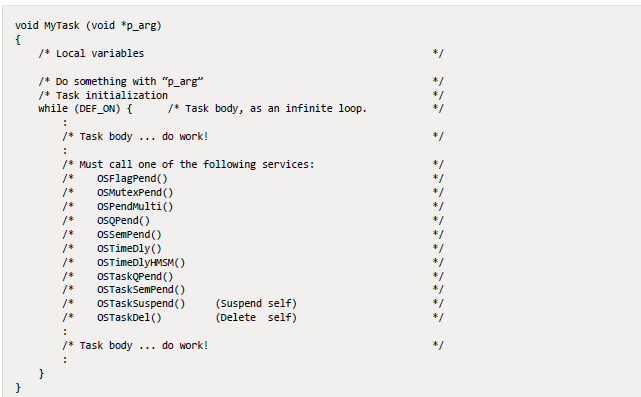
\includegraphics[scale=0.75]{008}}\par
而在一个应用程序等待某个中断发生时,使用的是EVENT FLAG机制。Even Flags是一系列的真值变量,应用程序可以调用OSFlagPend()函数等待一组真值变量中的任意一个变为真(OR)或等待所有变量均变为真(AND),而作为一个中断处理程序ISR,可以调用OSFlagPost()设置一组变量中的一个为真或假。因此,如果一个应用程序希望等待一个中断的发生,其可以设置一组事件标志组(EVENT FLAG),并等待其变为真。而对应的中断处理程序可以设置对应的Event Flag从而让应用程序进入Ready List并得知中断已经发生。如下图为一个典型的例子:

\centerline{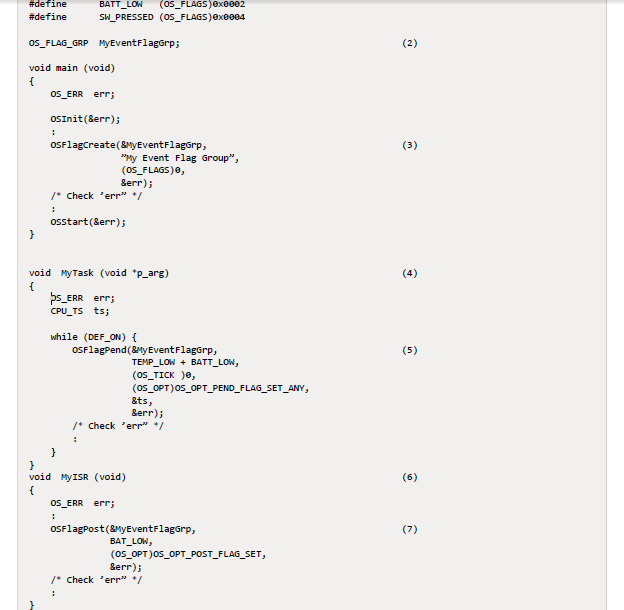
\includegraphics[scale=0.8]{009}}\par
在该任务中,如果发生了电池电量低的事件,MyTask就会从OSFlagPend()中返回并进行相应的处理。
\subsection{uC/OS II中中断处理程序的一般执行步骤}
 根据uC/OS官方提供的文档\cite{Manual},如下图为一般的嵌入式系统中中断的硬件连接。
 
\centerline{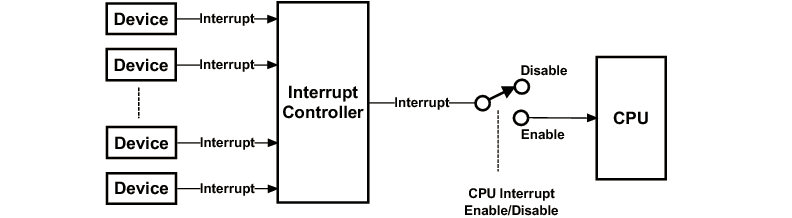
\includegraphics[scale=0.7]{010}}\par
   由于操作系统的存在,为了避免中断发生时发生进程上下文切换等事件的发生以及中断处理过程中又有中断发生,一般需要按照如下流程对中断进行处理。
   
\centerline{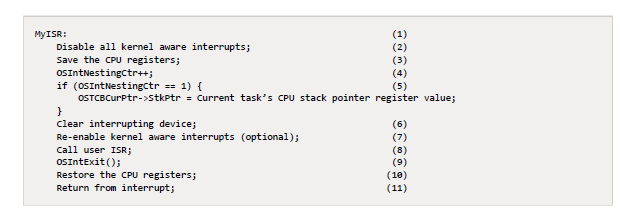
\includegraphics[scale=0.8]{011}}\par
首先需要关闭所有内核所能知晓的中断(对于有优先级的中断控制器,使用该种方法相当于没有使用优先级相关功能),以防止中断程序再次被中断。接下来保存CPU的所有寄存器在当前的任务栈上,标识自己进入了中断处理函数。如果自己是第一层中断,还需要保存当前任务的栈指针。截至将刚刚请求中断的设备的中断信号撤销,接着调用用户的中断程序(向其他程序发送事件标志Event Flag),接着就是一系列的退出动作,接着从中断处理程序中返回至操作系统。
\subsection{我们的移植方法}
在DA14580的SDK中,其已提供了部分中断处理程序,但由于其并没有操作系统的支持,所以在移植的过程中我们需按uC/OS II的要求进行一定的封装,即SDK提供的中断相当于user ISR,而我们则需在其基础上添加上关闭其他中断,保存CPU状态等内容即可。我们希望能从仅实现一个时钟中断开始(uC/OS需要),逐步向上添加蓝牙、UART、GPIO等相关内容。
\section{蓝牙协议栈的移植}
根据DA14580SDK提供的相关内容,其内涵一个RivieraWaves提供的ip核,并用.h导出了相关接口,如下图所示:

\centerline{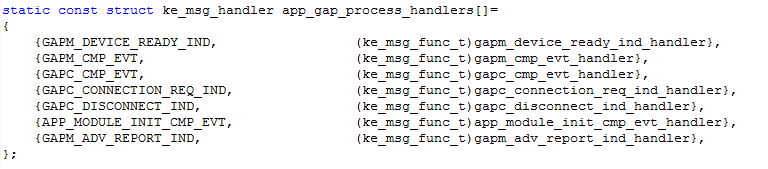
\includegraphics[scale=0.65]{012}}\par
上图描述了处理Generic Access Profile所需的函数,而这些函数最后在SDK的包装之下给用户提供了一个良好的接口,用户只需编写一个回调函数即可,如下图所示:

\centerline{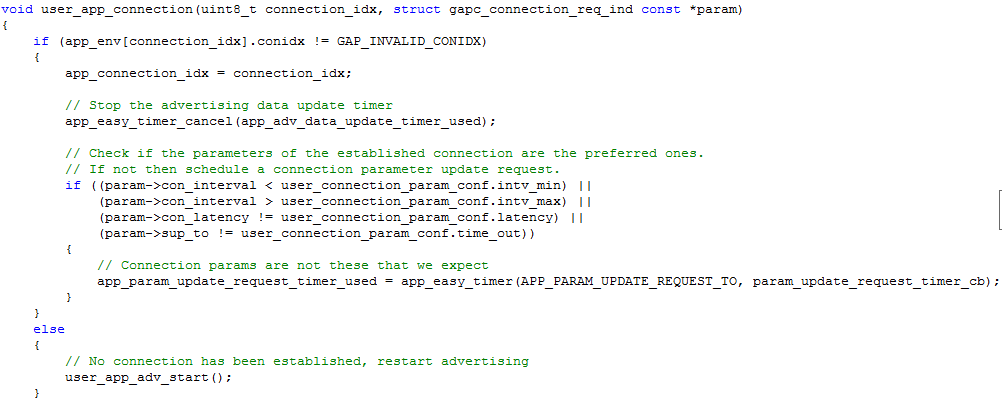
\includegraphics[scale=0.5]{013}}\par
而我们所需完成的是将上述蓝牙代码中的核心代码在uC/OS II上重新编写并将其中包含的原有SDK中的内容(如消息传递等)用uC/OS II中提供的机制实现。
\section{休眠功能的实现}
根据Dialog Semiconductor提供的资料,如下图所示,是能够使CPU进入休眠的主循环的一般模式:

\centerline{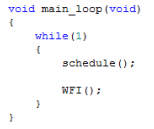
\includegraphics[scale=0.65]{014}}\par
但为了进入功耗更低的Extended Sleep Mode和Deep Sleep Mode,我们需要更详细的处理来替代简单地调用WFI()。WFI()为一个宏,指向一个函数\_WFI(),该函数调用ARM汇编指令wfi,其作用为使CPU停止运作直至新中断出现。因此,为了进入不同的休眠模式,我们需要在调用该宏前配置好各个组件的行为。具体需要执行的操作如下图:

\centerline{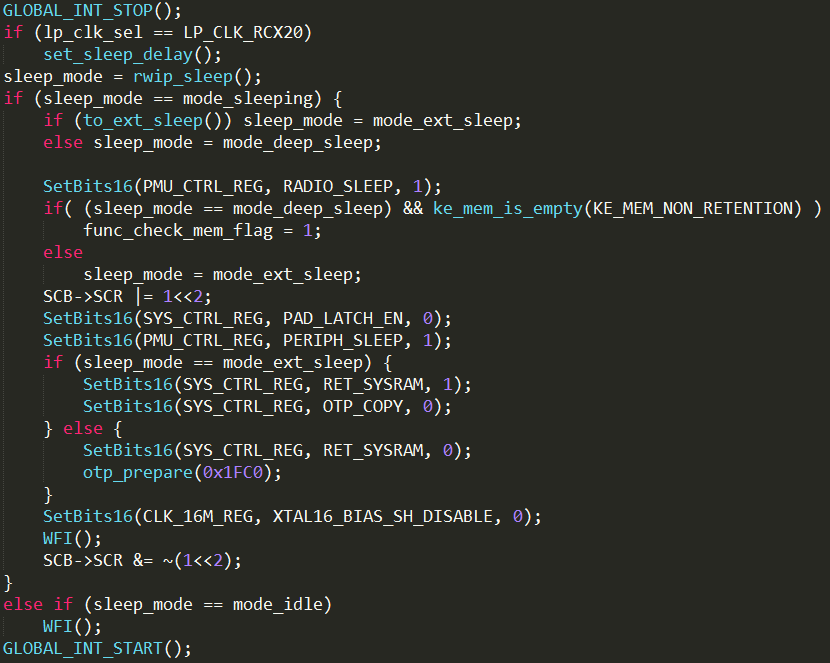
\includegraphics[scale=0.55]{015}}\par
上图是从SDK中的arch\_main.c中截下并整理的部分代码,应使用它们取代简单地调用WFI()。其中的宏和函数在SDK的其它部分均有定义。我们假设该设备同时只与一个蓝牙设备连接。

大致过程分如下几步:
\begin{enumerate}
\item 关闭中断。
\item 特殊情况处理:当低功耗时钟为RCX时钟时,为避免温度变化引起的时钟信号漂移,设定休眠延迟。
\item 调用RivieraWaves提供并由Dialog修改后的函数rwip\_sleep(),获取当前蓝牙模块状态所能允许的休眠模式:当蓝牙模块可停机时,为mode\_sleeping,否则为mode\_idle。
\item 当蓝牙模块可停机时,根据应用需求选择Extended Sleep Mode或Deep Sleep Mode。否则跳转至12。
\item 关闭无线电信号。
\item 当蓝牙协议栈内核的非保留堆不为空时,将Deep Sleep Mode改为Extended Sleep Mode以保留数据,否则标记func\_check\_mem\_flag以便其它部分查看。
\item 设置System Control Register以保证WFI()调用时进入休眠。
\item 启动PAD锁存器,关闭外设电源。
\item 根据不同的睡眠模式,关闭或保留SysRAM电源,准备恢复时OTP存储器读入SysRAM或关闭OTP存储器。
\item 关闭时钟信号,调用WFI()进入休眠。
\item 因中断被唤醒时,恢复System Control Register。跳转至13。
\item 蓝牙模块不可停机,直接调用WFI()停止CPU工作。
\item 重新启用中断。
\end{enumerate}
这其中需要注意的是,虽然调用WFI时全局中断均被禁用,但wfi指令本身无条件接收任何中断,因此不会导致无法被唤醒。而若在wfi前先启用中断,则在启用中断和调用wfi之间可能有中断的进入,导致不可预料的行为,这是不可行的。

但考虑到uC/OS II的设计并不存在一个主循环体,而是各个任务均为一个死循环,显然在每个任务中均人工添加休眠代码是不可行的——这会导致应用开发的不便。因此,我们考虑将上下文切换时当作主循环中两次schedule间的时机,在此时进行休眠。上下文切换的调用函数位于os\_cpu\_c.c中,如下图所示:

\centerline{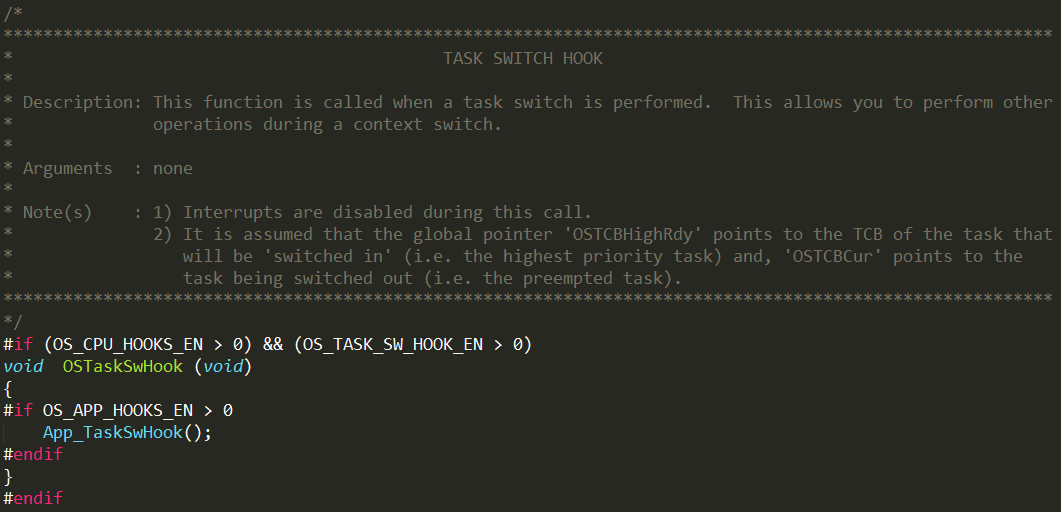
\includegraphics[scale=0.45]{016}}\par
只需在该函数体内加入上述代码,即可完成休眠工作。

唯一的问题在于休眠模式的选择。这一点我们选择先行实现Extended Sleep Mode,并将会在实际开发初步完成后通过测定功耗来确定是否需要考虑Deep Sleep Mode以通过降低效率来进一步降低功耗。
\section{创新点}
我们小组的工作的主要创新点主要有如下几点:
\begin{enumerate}
\item 向DA14580芯片中移植uC/OS

传统上,开发者基于由硬件厂商提供的SDK开发应用,这种开发方式有很多弊端。首先,直接将写好的应用烧录至开发板中导致只能运行单一应用,使得板子的功能单一。如果要将多种功能综合于同一应用中,必将大大增加代码的复杂性与开发难度,并且如果应用代码编辑不善极易使得系统资源利用不充分甚至导致各类错误的发生。此外这种开发方式使得扩展和更新应用变得困难并且延长了开发周期。

我们首先将uC/OS移植于DA14580蓝牙开发板,使其承担进程调度等相关功能。从而使得多应用并行运行成为可能。使得能够充分利用系统资源实现较为复杂的功能。通过uC/OS封装一部分底层接口,从而降低了应用开发难度,使得能够较快的实现功能扩展与更新。
\item 休眠功能的实现

当今制约蓝牙与许多嵌入式设备应用的关键点往往在于功耗问题。因此为了尽可能降低功耗,许多此类设备上并未安装完整的操作系统。我们将uC/OS移植进DA14580后,主要通过尽可能多的进入低功耗休眠模式从而使得平均功耗基本与传统方式相同。
因为uC/OS的设计中不存在主循环体而原SDK通过在循环体中调用相关函数实现。为避免重复在各个应用循环中添加相关调用造成的不便,我们创新性的提出了在上下文切换时处理休眠相关任务的解决方案。并且能够在Extended Sleep Mode和Deep Sleep Mode中进行合理选择,在功耗与性能之间达到更好的平衡。
\item 移植蓝牙协议栈

DA14580原设计内部存在一IP核提供蓝牙协议栈相关功能,通过将相关代码移植入uC/OS,可以通过操作系统来完成这些辅助工作。这样一方面能够更加高效的利用资源,同时也有利于后续的更新升级。
\end{enumerate}

\bibliography{report}
\bibliographystyle{plain}
\end{document}